\chapter{Physical Problem}
\label{PhysicalProblemChapter}
\lhead{Chapter 2. \emph{Physical Problem}} In this chapter, Maxwell's equations
of classical electrodynamics are introduced, both in integral and differential
forms. The wavelengths of interest are sufficiently large, with
respect to atomic scale variations in the medium, that a macroscopic approach is
justified and quantum mechanical effects are neglected. Constitutive
equations will be introduced for linear, isotropic material both with and
without dispersive effects. Following this, we introduce the Drude model and use it
to incorporate frequency-dependent interactions into Maxwell's
equations in a formulation suitable for efficient numerical calculation. The
conditions which must be satisfied at material interfaces will be derived and
alternative forms of Maxwell's equations discussed.

\section{Maxwell's equations}
The classical theory of electrodynamics decribes the behaviour evolution of
electromagnetic radiation using Maxwell's unification of the equations of
electrodynamics\cite{Balanis:ui,Jackson:490457}. The resulting coupled
equations, which govern the time evolution of electromagnetic waves, are known
collectively as Maxwell's equations and expressed in integral form and standard
units as
\begin{subequations}
  \begin{align}
    \int_{\partial S} \Etilde(\xbftilde,\ttilde) \cdot \vectdl  &= - \frac{d}{dt} \int_{S} \Btilde(\xbftilde,\ttilde) \cdot \vectdS, \label{eq:maxwell-faraday-integral} \\
    \int_{\partial S} \Btilde(\xbftilde,\ttilde) \cdot \vectdl &= \mu_0 \eps_0 \frac{d}{dt} \int_{S} \Etilde(\xbftilde,\ttilde) \cdot \vectdS +  \mu_0 \int_{S} \Jtilde(\xbftilde,\ttilde) \cdot \vectdS, \label{eq:maxwell-ampere-integral} \\
    \int_{\partial \Vol} \Dtilde(\xbftilde,\ttilde)\cdot\vectdS &= \int_\Vol \rho \,\dV, \label{eq:maxwell-gauss-integral} \\
    \int_{\partial \Vol} \Btilde(\xbftilde,\ttilde)\cdot\vectdS &= 0, \label{eq:maxwell-gauss-magnetism-integral}
  \end{align}
\end{subequations}
where $\xbftilde$ is the position vector, $\ttilde$ is time in seconds, $\eps_0$
is the permittivity of free space in farads per meter, $\mu_0$ is the
permeability of free space in henries per meter and the vectors
$\Etilde$, $\Htilde$, $\Dtilde$ and $\Btilde$ are used to denote respectively
the electric field, magnetic field, electric displacement and magnetic
induction. % QUOTE: both denote sources due to free charges in the system
$\Vol$ denotes any closed volume while the infinitesimal integration elements
$\vectdl$, $\vectdS$ and $\dV$ are respectively a line element, vector surface
element and volume element.
% "In regions where the material parameters are differentiable"... -> but hang
% on! The material parameters are not involved here. What restrictions are the
% for using Stokes' Theorem?
By applying Stokes' Theorem to~\eqref{eq:maxwell-faraday-integral}
and~\eqref{eq:maxwell-ampere-integral} and Gauss' law
to~\eqref{eq:maxwell-gauss-integral}
and~\eqref{eq:maxwell-gauss-magnetism-integral}, the equations in differential
form are readily obtained as
\begin{subequations}
  \label{eq:maxwells-equations-diff}
  \begin{align}
    \nablatilde \times \Etilde(\xbftilde,\ttilde) + \dpartttilde{\Btilde(\xbftilde, \ttilde)}&= \mathbf{0}, \label{eq:maxwell-faraday} \\
    \nablatilde \times \Htilde(\xbftilde,\ttilde) - \dpartttilde{\Dtilde(\xbftilde, \ttilde)}&= \Jtilde(\xbftilde,\ttilde), \label{eq:maxwell-ampere} \\
    \nablatilde \cdot \Dtilde (\xbftilde,\ttilde) &= \rho(\xbftilde,\ttilde), \label{eq:maxwell-gauss-1}, \\
    \nablatilde \cdot \Btilde (\xbftilde,\ttilde) &= 0, \label{eq:maxwell-gauss-2} .
  \end{align}
\end{subequations}
Where the operator $\nablatilde \times$ and $\nablatilde \cdot$ denote respectively taking the curl and taking the divergence, both with respect to the position vector $\xbftilde$.
The four equations in~\eqref{eq:maxwells-equations-diff} are known respectively
as Ampere's law with Maxwell's correction, Faraday's law, Gauss' law and Gauss'
law for magnetism. Maxwell's curl equations,~\eqref{eq:maxwell-ampere}
and~\eqref{eq:maxwell-faraday}, determine the evolution of the vector fields in
time, and Maxwell's divergence conditions,~\eqref{eq:maxwell-gauss-1}
and~\eqref{eq:maxwell-gauss-2}, are constraints on the vector fields which must
be satisfied at all times.

\subsection{Conservation of charge}
Conservation of charge can be derived directly from Maxwell's equations. The
vector identity
\begin{equation}
  \label{eq:vector-identity-1}
  \nablatilde \cdot ( \nablatilde \times \mathbf{A} (\xbftilde) ) = 0,
\end{equation}
which holds for any vector field $\mathbf{A}$, is substituted into the
expression obtained by taking the divergence of both sides of Ampere's
law,~\eqref{eq:maxwell-ampere}, giving:
$$
- \dpartttilde{( \nablatilde \cdot \Dtilde(\xbftilde,\ttilde) ) } = \nablatilde \cdot
\Jtilde(\xbftilde,\ttilde) .
$$
By substituting Gauss' law,~\eqref{eq:maxwell-gauss-1}, into this equation we
obtain the following conservation equation for charge
\begin{equation}
  \label{eq:maxwell-charge-conservation-2}
  \nablatilde \cdot \Jtilde(\xbftilde,\ttilde) + \dpartttilde{\rho (\xbftilde,\ttilde) } = 0 .
\end{equation}
Taking the divergence of Amperes law,~\eqref{eq:maxwell-ampere}, and removing
the curl term by recalling the identity~\eqref{eq:vector-identity-1}, results in
$$
\nablatilde \cdot \dpartttilde{ \Dtilde(\xbftilde, \ttilde)} = - \nablatilde \cdot
\Jtilde(\xbftilde,\ttilde),
$$
which can be rewritten using the conservation of charge
equation,~\eqref{eq:maxwell-charge-conservation-2}, as
$$
\nablatilde \cdot \dpartttilde{\Dtilde(\xbftilde, \ttilde)} = - \dpartttilde{ \rho
  (\xbftilde,\ttilde)}.
$$
Following a similar procedure using~\eqref{eq:maxwell-faraday} results in
$$
\nablatilde \cdot \dpartttilde{ \Btilde(\xbftilde, \ttilde)} = 0
$$

Thus provided the initial conditions satisfy equation Maxwell's divergence
conditions,~\eqref{eq:maxwell-gauss-1} and~\eqref{eq:maxwell-gauss-2}, and the
conservation of charge equation,~\eqref{eq:maxwell-charge-conservation-2}, is
satisfied at all times then if the system is evolved in time using Maxwell's
curl equations alone the divergence conditions will be implicitly satisfied at
all times.

\section{Constitutive equations}
\label{Ch:PhysicalProblem:ConstitutiveEquations}
Maxwell's equations in differential form,~\eqref{eq:maxwells-equations-diff},
are an underdetermined system of equations, with 4 equations and 6 unknowns. The
system of equations is closed by macroscopic constitutive laws, written as
% VIVA: this is not true for materials which exhibit ferromagnetic or
% ferroelectric behaviour - but this is a quantum effect, so outside of our
% classical scope. what are the constitutive laws in this case?
\begin{subequations}
  \begin{align}
    \Dtilde(\xbftilde,\ttilde) &= \eps_0 \Etilde(\xbftilde,\ttilde) + \Ptilde\left[ \Etilde, \Htilde, \xbftilde, \ttilde \right]  \label{eq:constitutive-general-E}\\
    \Btilde(\xbftilde,\ttilde) &= \mu_0 \Htilde(\xbftilde,\ttilde) + \Mtilde\left[ \Etilde, \Htilde, \xbftilde, \ttilde \right] \label{eq:constitutive-general-H}
  \end{align}
\end{subequations}
where $\Ptilde$, the polarisation density, and $\Mtilde$, the magnetisation
density, quantify the change in $\D$ and $\B$ resulting from the interaction
between the applied electromagnetic fields and the medium.
% However, for a given material the dependence may be non-local in space,
% non-local in time, non-linear, and/or anisotropic.
The polarisation and magnetisation densities for linear, isotropic and media
with frequency-independent material properties are described as
\begin{subequations}
  \begin{align}
    \Ptilde &= \ElecSuccept(\xbftilde) \Etilde(\xbftilde,\ttilde), \label{eq:elec-susceptibilities-definition-E} \\
    \Mtilde &= \MagSuccept(\xbftilde) \Htilde(\xbftilde,\ttilde) . \label{eq:elec-susceptibilities-definition-H} 
  \end{align}
\end{subequations}
where $\ElecSuccept$, the electric suceptibility, and $\MagSuccept$, the
electric susceptibility, are a measure of polarisation or magnetisation of the
medium in response and applied fields.
Using~\eqref{eq:elec-susceptibilities-definition-E}
and~\eqref{eq:elec-susceptibilities-definition-H}, the constitutive equations,
shown in~\eqref{eq:constitutive-general-E}
and~\eqref{eq:constitutive-general-H}, can be rewritten in the simple form
\begin{subequations}
  \label{eq:constitutive-linear}
  \begin{align}
    \Dtilde(\xbftilde,\ttilde) = \eps_0 \eps_r(\xbftilde) \Etilde(\xbftilde,\ttilde), \label{eq:constitutive-linear-D} \\
    \Btilde(\xbftilde,\ttilde) = \mu_0 \mu_r(\xbftilde) \Htilde(\xbftilde,\ttilde),\label{eq:constitutive-linear-B}
  \end{align}
\end{subequations}
where the material response is completely characterised by two dimensionless
scalars $ \eps_r, \mu \in \Real$, known respectively as the permittivity and the
relative permeability, given by $\eps_r \equiv 1 + \ElecSuccept $ and $\mu_r
\equiv 1 + \MagSuccept $.
% TODO - cite{Maier:5SXqSjV8} -> copied

\subsection{Dispersive Drude Media}
Most media exhibits frequency dependence of both $\eps_r$ and $\mu_r$, a
phenomena known as dispersion, which arises due to the finite time the medium needs to
repond to changes in applied electromagnetic fields.
Whilst dispersive effects are generally neglected in simulations of dielectrics, many metals
of interest in photonics, such as gold, silver and aluminum,
have strongly frequency dependent relative permittivities in the visible and infra-red
regions of the electromagnetic spectrum\cite{Ordal:1983bg}. This is a
consequence of the finite time required for charged particles in the medium to
reach a equilibrium positions in the presence of a changing applied
electromagnetic field. In these cases, the electric susceptibility can
no longer be written as a function of $\xbftilde$ only, but is expressed
as convolution integrals in time\cite{Jackson:490457}.
% VIVA: article - A comparison of numerical techniques for modeling
% well
For metals where the effects of interband electron transitions are negligible, a
mechanical model based on the Drude model of solids is
sufficient\cite{taflove2013advances}. For more complex material interactions however,
a more sophisticated model such as the Drude-Lorentz model\cite{Fox:2001wm,Taflove:1989ds}
or approaches based on the $Z$-transform\cite{sullivan1996z} may be used.
We restrict the follow discussion to media and frequency ranges where
magnetisation effects are frequency-independent, and thus~\eqref{eq:constitutive-linear-B} remains valid,
and where polarisation can be approximated by a single-pole Drude model.

%% *** ## "Polarisation density also describes how a material responds to an
%% applied electric field as well as the way the material changes the electric
%% field, and can be used to calculate the forces that result from those
%% interactions."
% ...based on the kinetic theory of gases,
%
% *** "The induced polarisation due to frequency-dependent electron movement
% leads to a frequency-dependent polarisation (dispersion)" - ref Maier
%
% Electron-ion collisions are random events, with a probability $dt / \tau$ (tau
% is the inv of gamma) - following which the electron velocities are independent
% of velocities prior to collision.
A Drude medium is composed of a lattice of fixed-position, positively charged
ions bound by a delocalised sea of valence band free
electrons\cite{Ashcroft:2005wp,Bandyopadhyay:1503732}. The free electrons,
following the kinetic theory of ideal gases, are non-interacting, independent
particles, described by Newtonian mechanics. In the presence of the electric
field, $\Etilde$, the ions remain fixed and only the free electrons are
displaced from their zero-field equilibrium positions. In the Drude model
polarisation arises from two independent sources: a frequency-independent background polarisation,
$\PtildeInf$, due to the fixed-position charged ions, and
a frequency dependent free electron polarisation, $\PtildeElec$, due to the delocalisation of
free electrons in the presence of an electric field.
Thus we begin by writing~\eqref{eq:constitutive-general-E} in the frequency domain as
\begin{align}
  \hat{\Dtilde}(\xbftilde,\omega) &= \eps_0 \hat{\Etilde}(\xbftilde, \omega) + \PtildeInfFreq + \PtildeElecFreq(\xbftilde,\omega) ,
                                    \label{eq:constitutive_equations_drude_model}
\end{align}
where $\omega$ is the frequency variable and a circumflex denotes the frequency domain representation of a time domain quantity, such that
$$
\hat{\Box}(\xbftilde,\omega) = \int_{-\infty}^{+\infty} \Box(\xbftilde,\ttilde) e^{-i \omega t} dt
$$
where the real-valued function $\Box$ of the temporal variable, $\ttilde \in \Real$, has
been written as the complex valued function $\hat{\Box}$ of angular frequency, $\omega \in \Real$, which is related to frequency, $f$, by $\omega = 2 \pi f$. Note in particular that $- i \omega
\hat{\Box}(\xbftilde,\omega) = \dpartt{ \Box(\xbftilde,\ttilde) }$.
Since $\PtildeInfFreq$ is frequency-independent, following the procedure from~\autoref{Ch:PhysicalProblem:ConstitutiveEquations}, we rewrite~\eqref{eq:constitutive_equations_drude_model} as
\begin{equation}
\hat{\Dtilde}(\xbftilde,\omega) = \eps_0 \eps_{\infty} \hat{\Etilde}(\xbftilde, \omega) + \hat{\Ptilde}_e(\xbftilde,\omega) ,
\end{equation}
where $\eps_{\infty} \equiv 1 + \ElecSucceptInf $ is the permittivity in the infinite frequency limit, and $\ElecSucceptInf$ is defined by 
$\PtildeInfFreq \equiv \eps_0 \ElecSucceptInf \hat{\Etilde} $.
Transforming~\eqref{eq:constitutive_equations_drude_model} directly to the time
domain would lead to a convolution integral, which presents challenges for
numerical simulation\cite{kelley1996piecewise}. We instead follow the so called
Auxiliary Differential Equation (ADE)
approach\cite{Taflove:1989ds,Niegemann:2009uv,Ji:2007dl,okoniewski1997simple,kashiwa1990treatment}, and
multiply~\eqref{eq:constitutive_equations_drude_model} by $ -i \omega$ prior to
applying the transform, to obtain a constitutive relation as an ordinary differential equation
\begin{equation}
  \label{eq:constitutive_equations_drude_model_derivative_TD}
  \dodettilde{ \Dtilde (\xbftilde,\ttilde) }= \eps_0 \eps_{\infty} \dodettilde{ \Etilde (\xbftilde, \ttilde) } + \Jtildep(\xbftilde,\ttilde) .
\end{equation}
where, $\Jtildep$, the current due to free electron polarisation, has been
defined as $ \Jtildep(\xbftilde,\ttilde) = - \dpartt{\Ptilde}_e(\xbftilde,\ttilde) $.
% TODO - check that the - is correct in this definition, and that J is defined
% in the opposite direction to P
By substitution into Ampere's law,~\eqref{eq:maxwell-ampere}, we obtain the
expression
\begin{align}
  \nablatilde \times \Htilde(\xbftilde,\ttilde) - \dpartttilde{\Dtilde_{\infty}(\xbftilde, \ttilde)} &= \Jtilde(\xbftilde,\ttilde) + \Jtildep(\xbftilde,\ttilde) , \label{eq:drude-ampere}
\end{align}
where, to maintain consistency with dispersion-free form of Maxwell's equations~\eqref{eq:maxwells-equations-diff} we have defined $\Dtilde_{\infty} \equiv \eps_0 \eps_{\infty} \Etilde$, as the electric
displacement in the infinite frequency limit.

To close the system of equations an expression for $\Jtildep$ is required. Since
this is the current due to movement of free electrons, we begin by writing the
Newtonian equation of motion of a free electron in the presence of an applied
electric field, as
\begin{equation}
  \frac{d^2 \xbftilde(\ttilde) }{dt^2}+ \gamma \frac{d \xbftilde(\ttilde) }{dt}= \frac{q}{m_e}\Etilde(\xbftilde(\ttilde),\ttilde),
  \label{eq:equations-of-motion-electron}
\end{equation}
where $\gamma$ is a damping coefficient or collision frequency, $m_e$ is the
mass of an electron, $q$ is the charge of an electron,
$\Etilde(\xbftilde,\ttilde)$ is the applied electric field and $\xbftilde$ is
the displacement of the electron from its zero-field equilibrium position. Given
that the polarisation field due to electron movement is given by $
\PtildeElec(\ttilde) = - n q \xbftilde(\ttilde)$, where $n$ is the electron
density in the medium, then~\eqref{eq:equations-of-motion-electron} can be
rewritten as
\begin{equation}
  \label{eq:polarisation-from-P}
  - \frac{d^2 \PtildeElec(\ttilde) }{dt^2} - \gamma \frac{d \PtildeElec(\ttilde) }{dt} = \eps_0 \plasfreq^2 \Etilde(\xbftilde(\ttilde),\ttilde),
\end{equation}
where $\plasfreq = \sqrt{\frac{n q^2}{m_e \eps_0}}$ is known as the plasma
frequency.
% We consider a single frequency in the frequency domain by selecting a
% monochromatic field of the form
%$$
%\Etilde(\xbftilde,\ttilde) = \hat{\mathbf{E_0}} e^{- i \omega \ttilde}
%$$
%with a known angular frequency $w$ and constant amplitude $\hat{\Etilde}$.
%
from the definition of $\Jtildep$,~\eqref{eq:polarisation-from-P} can be written as
\begin{equation}
  \dpartttilde{\Jtildep(\xbftilde,\ttilde)} + \gamma \Jtildep(\xbftilde) = \eps_0 \plasfreq^2 \Etilde(\xbftilde,\ttilde).
  \label{eq:pol-current-ADE}
\end{equation}

Maxwell's curl equations and constitutive equations in a Drude dispersive medium,
are given by
\begin{subequations}
  \label{eq:dispersive-maxwell-system}
  \begin{align}
    \nablatilde \times \Etilde(\xbftilde,\ttilde) + \dpartttilde{ \Btilde(\xbftilde, \ttilde)}&= 0, \\
    \nablatilde \times \Htilde(\xbftilde,\ttilde) - \dpartttilde{ \Dtilde_{\infty}(\xbftilde, \ttilde) }&= \Jtilde(\xbftilde,\ttilde) - \Jtildep(\xbftilde,\ttilde), \\
    \Dtilde_{\infty}(\xbftilde,\ttilde) &= \eps_0 \eps_{\infty}(\xbftilde) \Etilde(\xbftilde,\ttilde), \\
    \Btilde(\xbftilde,\ttilde) &= \mu_0 \mu_r(\xbftilde) \Htilde(\xbftilde,\ttilde), \\
    \frac{d \Jtildep(\xbftilde)}{dt} + \gamma \Jtildep(\xbftilde) &= - \eps_0 \plasfreq^2 \Etilde(\xbftilde, \ttilde) . \label{eq:maxwell-dispersive-ADE}
  \end{align}
\end{subequations}
We note that these equations reduce to the non-dispersive case, given
in~\eqref{eq:maxwell-ampere},~\eqref{eq:maxwell-faraday} and~\eqref{constitutive-linear} 
in the infinite frequency limit.

Some insight into the behaviour of Drude metals can be obtained by looking at
the relative permittivity obtained in the frequency domain.
First,~\eqref{eq:polarisation-from-P-FD} can be rearranged to obtain the
polarisation due to free electrons in the frequency domain,
\begin{equation}
  \hat{\Ptilde}_e = - \frac{\eps_0 \plasfreq^2}{\omega^2 - i \omega \gamma } \hat{\Etilde}(\omega) .
  \label{eq:polarisation-field-freq-domain}
\end{equation}
Using this expression,~\eqref{eq:constitutive_equations_drude_model} may be
rewritten explicitly in the frequency domain as
\begin{equation}
  \begin{split}
    \hat{\Dtilde}(\xbftilde,\omega) &= \eps_0 \left( \eps_{\infty} - \frac{\plasfreq^2 }{\omega^2 - i \omega \gamma } \right) \hat{\Etilde}(\omega) \\
    &= \eps_0 \hat{\eps}_r (\omega) \hat{\Etilde}(\omega) ,
  \end{split}
\end{equation}
where $\hat{\eps}_r(\omega)$ is the effective permittivity of the metal. Figure
\ref{fig:read-and-imag-effective-permittivity} shows the real and imaginary
parts of $\hat{\eps}_r$, given by
\begin{subequations}
  \begin{align}
    Re\{ \hat{\eps}_r \} &= \eps_{\infty} - \frac{\plasfreq^2}{\omega^2 + \gamma^2}, \\
    Im\{ \hat{\eps}_r \} &= \frac{\gamma \plasfreq}{\omega ( \omega^2 + \gamma^2) } ,
  \end{align}
\end{subequations}
plotted against normalised angular frequency $\omega / \plasfreq$. We observe
that at higher frequencies, due to reduced electron motion, the non-dispersive
dielectric behaviour is recovered as $Re\{\hat{\eps}_r\} \to \eps_{\infty}$ and
$Im\{\hat{\eps}_r\} \to 0$. For frequencies below $\plasfreq$ however, the real
and imaginary parts of the permittivity diverge significantly from the
dispersive values. The positive values of the imaginary part result in an
attenuation of the electric field amplitude in this region.

\begin{figure}[htbp!]
  \begin{center}
    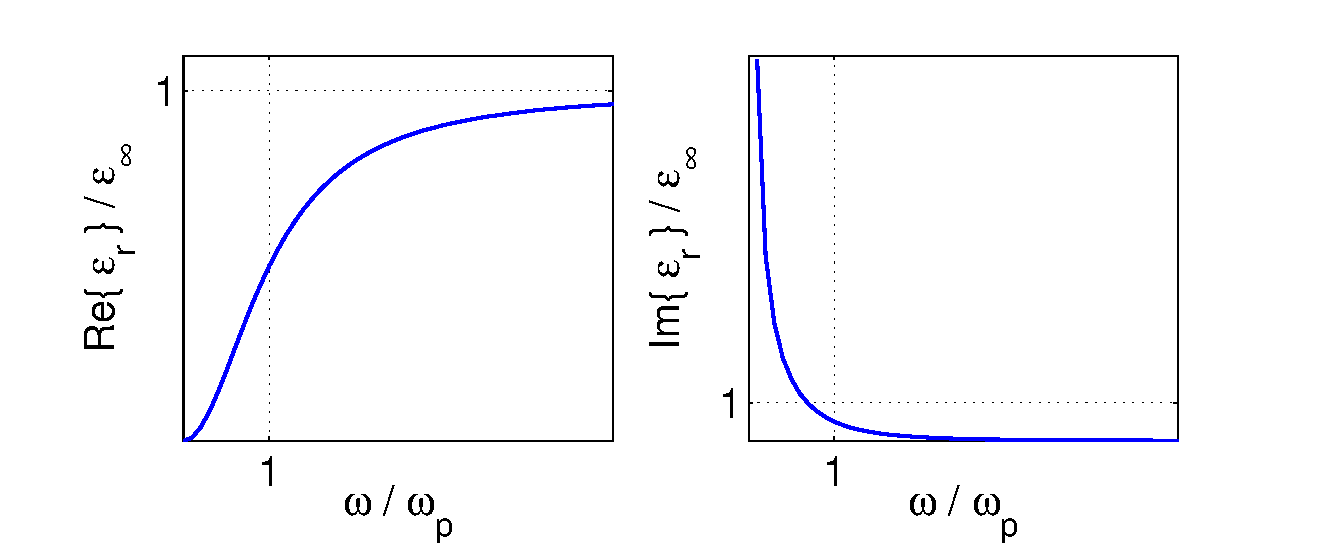
\includegraphics[scale=0.7]{Figures/Chapters/PhysicalProblem/drudePermittivity}
  \end{center}
  \caption{The real (left) and imaginary (right) parts of the dispersive
    frequency domain relative permittivity, $\hat{\eps}_r$, as obtained from
    Drude model.}
  \label{fig:read-and-imag-effective-permittivity}
\end{figure}


%%%%%%%%%%%%%%%%%%%%%%%%%%%%%%%%%%%%%%%%%%%%%%%%%%%%%%%%%%%%%%%%%%%%%%%%%%%%%%%%%%%%%%%%%%%%%%%%%%%%%%%%%%%%%%%%%%%%%%%%%%%%%%%%%%%%%%%%%%%%%%%%%%%%%
% More Dude Model Stuff
%%%%%%%%%%%%%%%%%%%%%%%%%%%%%%%%%%%%%%%%%%%%%%%%%%%%%%%%%%%%%%%%%%%%%%%%%%%%%%%%%%%%%%%%%%%%%%%%%%%%%%%%%%%%%%%%%%%%%%%%%%%%%%%%%%%%%%%%%%%%%%%%%%%%%
%
% TODO - direct quote - IntriaPaper DGTD dispersive
%
% When subjected to a constant external electric field $\Etilde$ the
% displacement of the heavy valence ions from their equilibtrium position is
% assume to be negligable whilst the electrons move significantly from their
% equilibrium position in response to an externally applied field. This results
% in an additional electric field $\Ptilde$ due to material response to the
% applied field $\Etilde$ orientated in the opposite direction resulting in a
% total field given by the electric displacement field $\Dtilde$ where:
% 
%  $$
%  \Dtilde = \eps_0 \Etilde + \Ptilde
%  $$
% 
%  Note that usually the signs of $\Ptilde$ and $\Etilde$ will be opposite -
%  resulting in an induced field that opposes the applied field and
%  consequentially a reduced field in the medium.
% 
%  %  TODO: Is it accurate to describe the displacement electric field as the
%  %  total electric field....?
% 
%  For a constant or slow-varying field with respect to the material response
%  time $\tau$ the polarisation of the material $\Ptilde$ will be proportional
%  to the applied electric field and can be described as a constant of
%  proportionality $\chi$, known as the electric susceptibility which describes
%  how susceptible the material is to polarisation. $\Ptilde$ can be written as:
% 
%  $$
%  \Ptilde = \chi \Etilde
%  $$
% 
%  $\chi$ is not always constant - and in general is a tensor.
% 
%  Furthermore the movement of electrons from their zero-field equlibrium
%  positions to the equilibrium positions under the applied field $\Etilde$
%  could take some finite time $\tau$ (characteristic time). For an applied
%  electric field $\Etilde$ which is changing sufficiently quickly this time
%  needs to be accounted for and $\chi$ may not be described as simply by a
%  constant since it clearly depends on the history of the mediums polarisation.
% 
%  TODO - derivation from equations of motion to conservation form....find a
%  nice way of doing this....
%
%
%
%  Even More Dude Model Stuff
%%%
%%%  Consider a medium under a constant external electric field $\Etilde$. Free
%%%  charged particles or charge dipoles in a material are subject to an applied
%%%  force. The equilibrium position of positive and negative charges will be
%%%  different to zero-field equilibrium positions and a net dipole moment, and
%%%  consequentially an electric field, is established. The electric
%%%  displacement, $D$, has a contribution due to polarisation of the material,
%%%  $P$, and~\eqref{eq:contitutive-linear-non-dispersive-1} is modified as
%%%
%%%   $$
%%%   \Dtilde(\mathbf{r},\ttilde) = \eps \Etilde(\mathbf{r},\ttilde) +
%%%   \Ptilde(\mathbf{r},\ttilde) ,
%%%   $$
%%%
%%%   In a changing applied field the movement of charges from a previous
%%%   equlibrium state to a subsequent equilibrium state could take some finite
%%%   time. Since this depends on the current state of polarisation the time
%%%   required to reach a new polarisation state is dependent not only on the
%%%   current applied field but also the history of the polarisation of the
%%%   medium. The material polarisation field $P$ can be written as
%%%
%%%   \begin{equation}
%%%   \Ptilde(\mathbf{r},\ttilde) = \eps_0 \int_{-\infty}^{+\infty} d \mathbf{r}' \int_{-\infty}^{\ttilde} dt' \chi (\mathbf{r} - \mathbf{r}', \ttilde - \ttilde') \cdot \Etilde(\mathbf{r}', \ttilde')
%%%   \label{eq:dispersive-convolution-integral}
%%%   \end{equation}
%%%
%%%
%%%   In the time domain the constitutive equations for dispersive materials
%%%   become non-local in time. The problem can be treated more naturally in the
%%%   frequency domain, where the material response depends on the applied
%%%   frequency. Then~\eqref{eq:contitutive-linear-non-dispersive-1} can be
%%%   written as:
%%%
%%%   \begin{equation}
%%%     \Dtilde(\omega) = \eps(\omega) \Etilde
%%%   \end{equation}
%%%
%%%
\section{Dimensionless form}

% "\eps_0 and \mu_0 introduces an arbitraryness of dimension which we exploit
% for the dimensionless form"
Maxwell's equations are not invariant under change of units, with the constants
$\eps_0$, $\mu_0$ and changing value and position. Unit systems in common
use include the SI units used above, Gaussian units, Lorentz-Heaviside units and
Planck units. In particular, for numerical simulations, a dimensionless unit
system is commonly used to avoid rounding errors in floating point arithmetic.
Maxwell's equations can be obtained in dimensionless form by scaling length and
time by an arbitrary characteristic length, $L$. The following changes of
variable are introduced:
\begin{align}
  \label{eq:dimensionless-scaling-1}
  \xbf &= \frac{\xbftilde}{\charLen}, &  \
                                        t &= \frac{\czero \ttilde}{\charLen}, &  \
                                                                           \plasfreq &= \frac{\plasfreqtilde \charLen}{\czero}, & \
                                                                                                                                  \gamma &= \frac{\gammatilde \charLen}{\czero},
\end{align}
where $\czero = ( \eps_0 \mu_0 )^{-\frac{1}{2}}$ is the speed of light in vacuum
in SI units, and the quantities $\xbf$ and $\t$ have been chosen such that the
dimensionless speed of light in vacuum is unity. Additionally, electromagnetic
field strengths and currents may be scaled by a characteristic field strength,
$\E_0$, by introducing the following dimensionless variables:
\begin{align}
  \label{eq:dimensionless-scaling-2}
  \E &= \Etilde, &  \
                   \H &= \intImpFS \Htilde, &  \
                                              \J &= \charLen \intImpFS \Jtilde, & \
                                                                                  \J_p &= \charLen \intImpFS \Jtilde_p,
\end{align}
% note - could also scale all of these values with E_0
where $\eta_0 = \sqrt{\mu_0 / \eps_0}$ is the intrinsic impedence of free space.
Derivatives with respect to $\ttilde$ and $\xbftilde$ are transformed as
\begin{align}
  \label{eq:dimensionless-scaling-3}
  \dpartttilde{\Box} &= \frac{\czero}{\charLen}\dpartt{\Box}, & \
                                                        \dpartxtilde{\Box} &= \frac{1}{\charLen}\dpartx{\Box}
\end{align}
By substitution of~\eqref{eq:dimensionless-scaling-1}
and~\eqref{eq:dimensionless-scaling-2} into Maxwell's curl
equations,~\eqref{eq:maxwell-ampere} and~\eqref{eq:maxwell-faraday}, we obtain
the curl equations modified for dispersive materials in dimensionless form:
\begin{subequations}
  \label{eq:dimensionless-maxwell}
  \begin{align}
    \nabla \times \E(\xbf,\t) + \dpartt{\B(\xbf, \t) } &= 0, \\
    \nabla \times \H(\xbf,\t) - \dpartt{ \D_{\infty}(\xbf, \t) } &= \J(\xbf,\t) - \J_p(\xbf,\t), \\
    \D_{\infty}(\xbf,\t) &= \eps_{\infty}(\xbf) \E(\xbf,\t), \\
    \B(\xbf,\t) &= \mu_r(\xbf) \H(\xbf,\t), \\
    \frac{d \J_p(\xbf,\t)}{d\t} + \gamma \J_p(\xbf,\t) &= - \omega_p^2 \E(\xbf,\t),
  \end{align}
\end{subequations}
where $\DInf$ and $\B$ are the appropriately scaled values of
$\DtildeInf$ and $\Btilde$.
Note that the non-dispersive form may be recovered in
the infinite frequency limit, where $\J_p = 0$, $\eps_{\infty} = \eps_r$
and $\DInf = \D$
equations,~\eqref{eq:maxwells-equations-diff}, to obtain the equivalent
non-dispersive dimensionless form.

\section{Conservation form}

% *** EVERYTHING WRITTEN AS FREE SPACE - \mu = 1 probably ok for my examples but
% \eps != 1 ***
The dispersive form of Maxwell's equations in dimensionless
form,~\eqref{eq:dimensionless-maxwell}, can be conveniently rewritten as a
linear, hyperbolic conservation law\cite{Godlewski:2013tj,LeVeque:2002vc}
% TODO - Ruben: need to show that system is hyperbolic (and linear?)
\begin{equation}
  \dpartt{ \, \USoltn} + \sum_{k=1}^{nsd} \frac { \partial \, \Flux_k(\USoltn) }{ \partial x_k } = \maxwellSource\,(\USoltn) \: ,
  \label{eq:maxwell-curl-equations-conservation-form}
\end{equation}
where $nsd$ denotes the number of spatial dimensions. The vector of unknowns,
$\USoltn$, the flux vectors, $\Flux_k$, and the source $\maxwellSource$ are
given by
\begin{equation*}
  \begin{array}{c}
    \USoltn =
    \begin{pmatrix}
      \eps_{\infty} E_1, \: \eps_{\infty} E_2 , \: \eps_{\infty} E_3 , \: \mu
      H_1 , \: \mu H_2 , \: \mu H_3 , \: J^p_1 , \: J^p_2 , \: J^p_3
    \end{pmatrix}^T,
    \\
    \Flux_1 =
    \begin{pmatrix}
      0 ,\: H_3 ,\: -H_2 ,\: 0 ,\: -E_3 ,\: E_2 ,\: 0 ,\: 0 ,\: 0
    \end{pmatrix}^T , \\

    \Flux_2 =
    \begin{pmatrix}
      - H_3 ,\: 0 ,\: H_1 ,\: E_3 ,\: 0 ,\: -E_1 ,\: 0 ,\: 0 ,\: 0
    \end{pmatrix}^T , \\

    \Flux_3 =
    \begin{pmatrix}
      H_2 ,\: -H_1 ,\: 0 ,\: -E_2 ,\: E_1 ,\: 0 ,\: 0 ,\: 0 ,\: 0
    \end{pmatrix}^T , \\

    \maxwellSource =
    \begin{pmatrix}
      J_1 + J^p_1 ,\: J_2 + J^p_2 ,\: J_3 + J^p_3 ,\: 0 ,\: 0 ,\: 0 ,\: \omega^2
      \: E_1 - \gamma J^p_1 ,\: \omega^2 \: E_2 - \gamma J^p_2 ,\: \omega^2 \:
      E_3 - \gamma J^p_3
    \end{pmatrix}^T,

  \end{array}
\end{equation*}

where $E_k$, $H_k$ and $J^p_k$ are the $k$th spatial components of the
dimensionless intensity vectors of electric field, magnetic field and the
polarisation current, respectively. The material parameters $\eps$, $\mu$,
$\omega$ and $\gamma$ are the electric permittivity, magnetic permeability,
plasma frequency and electron damping coefficient, respectively. The same form
may be used for non-dispersive cases, by setting $J^p_k = 0 \; \forall \; k$ and
setting $\eps_{\infty} = \eps_{r}$. The equations can be written in quasilinear form
\begin{equation}
  \label{eq:1}
  \dpartt{\USoltn}  + \AQuasiLinear_k\dpart{\xbf_k}{\USoltn} = \AQuasiLinear_s \USoltn  \;\;\;k = 1...\nsd
\end{equation}
where, in three dimensions

\begin{align}
\AQuasiLinear_k = 
    \begin{pmatrix}
      \zerov & \RQuasiL_{k} & \zerov \\
      -\RQuasiL_{k} & \zerov & \zerov \\
      \zerov & \zerov & \zerov \\
    \end{pmatrix}
  \: \:
\textrm{and}\;\;\;
\AQuasiLinear_s = 
    \begin{pmatrix}
      \zerov  & \zerov & -\IdentityVect\\
      \zerov & \zerov & \zerov \\
      -\plasfreq \IdentityVect & \zerov & - \gamma \IdentityVect \\
    \end{pmatrix}
\end{align}
with
\begin{align}
\RQuasiL_1 = 
    \begin{pmatrix}
      0 & 0 & 0 \\
      0 & 0 & 1 \\
      0 & -1 & 0 \\
    \end{pmatrix} ,
  \: \:
  &
\RQuasiL_2 = 
    \begin{pmatrix}
      0 & 0 & -1 \\
      0 & 0 & 0 \\
      1 & 0 & 0 \\
    \end{pmatrix}
  &
  \textrm{and   } \:\:\:
  &
\RQuasiL_3 = 
    \begin{pmatrix}
      0 & 1 & 0 \\
      -1 & 0 & 0 \\
      0 & 0 & 0 \\
    \end{pmatrix}
  &
\end{align}

% TODO - quasilinear form for TE and TM

\section{Reduction to 2 dimensions}
\subsection{TE and TM modes}
For a physical system where the electric field is translationally invariant in
the $z$-direction, the derivatives with respect to $z$ are zero. Maxwell's
equations are decoupled into two sets of coupled equations with three unknowns
each. The resulting modes in dimensionless form, accounting for dispersion with
the Drude model, are known as the $TE_z$ mode, given by

\begin{equation*}
  \begin{array}{ccccc}
    \USoltn_1 = \begin{pmatrix} \eps E_1 \\ \eps E_2 \\ \mu H_3 \\ J^p_1 \\  J^p_2 \end{pmatrix} ,
 &
   \Flux_1 = \begin{pmatrix} 0 \\ H_3 \\ E_2 \\ 0 \\  0 \end{pmatrix} ,
 &
   \Flux_2 = \begin{pmatrix} - H_3 \\ 0 \\ -E_1 \\ 0 \\ 0 \end{pmatrix} ,
 &
   \maxwellSource = \begin{pmatrix} J_1 + J^p_1 \\ J_2+ J^p_2 \\ 0 \\ \omega^2 \, E_1 - \gamma J^p_1 \\  \omega^2 \, E_2 - \gamma J^p_2 \end{pmatrix} ,
  \end{array}
  \:
\end{equation*}

and the $TM_z$ mode, given by

\begin{equation*}
  \begin{array}{ccccc}
    \USoltn = \begin{pmatrix} \eps E_3 \\ \mu H_1 \\ \mu H_2 \\ J^p_3 \end{pmatrix} ,
 &
   \Flux_1 = \begin{pmatrix} -H_2 \\ 0 \\ -E_3 \\ 0 \end{pmatrix} ,
 &
   \Flux_2 = \begin{pmatrix} H_1 \\ E_3 \\ 0 \\ 0 \end{pmatrix} ,
 &
   \maxwellSource = \begin{pmatrix} J_3 + J^p_3 \\ 0 \\ 0 \\ \omega^2 \, E_3 - \gamma J^p_3 \end{pmatrix} .
  \end{array}
  \:
\end{equation*}

In particular, radiation which is quantised by confinement in a waveguide can be
described by the $TE_z$ or $TM_z$ modes.
% In practice a system which can be approximated as having infinite extent in
% one direction can be approximated by a translationally invariant electric
% field in one direction.

\subsection{2D compact form}

Several physical systems, notably wave guides, may have known modal dependence
in a given direction. The compact form of Maxwell's equations was introduced by
Xiao\cite{Xiao:1992be} to allow a full wave analysis of Maxwell's equations in
waveguides using only a 2-dimensional mesh. The variation of fields in the
$z$-direction is assumed to be of the form
\begin{equation}
  \USoltn(x_1,x_2,x_3) = \USoltn_{12}(x_1, x_2,t) e^{-i \beta_z x_3},
  \label{eq:compact2D-zdep}
\end{equation}
where $\beta_z$ is the wave propagation constant in the $z$-direction. By
substitution into Maxwell's non-dispersive
equations,~\eqref{eq:maxwell-curl-equations-conservation-form}, with
$\maxwellSource = 0$, the system of equations obtained can be written in compact
form\cite{}, resulting in the following expressions for $\USoltn$,$\Flux_{k}$
and $\maxwellSource$
\begin{equation*}
  \begin{array}{ccccc}
    \USoltn = \begin{pmatrix} \eps_{\infty} E_1 \\ \eps_{\infty} E_2 \\ \eps_{\infty} E_3 \\ \mu H_1 \\ \mu H_2 \\  \mu H_3  \end{pmatrix} ,
 &
   \Flux_1 = \begin{pmatrix} 0 \\ H_3 \\ -H_2 \\ 0 \\ -E_3 \\ E_2  \end{pmatrix} ,
 &
   \Flux_2 = \begin{pmatrix} - H_3 \\ 0 \\ H_1 \\ E_3 \\ 0 \\ -E_1 \end{pmatrix} ,
 &
   \maxwellSource = \begin{pmatrix} H_2 \\ -H_1 \\ 0 \\ -E_2 \\ E_1 \\ 0 \end{pmatrix} i \beta_z ,
  \end{array}
  \:
\end{equation*}

where the fields $E_k'$, $H_k'$ do not contain any dependence on $z$. Note that
the expression for $\maxwellSource$ is now complex, however for scalar permittivities the system can be solved by taking only
the real part\cite{zhao1997relationship,pile2005compact}.
% TODO - Ruben : the citations here might need to be changed
%
% E Blank In case a numerical scheme is applied to discretize the curl-equations, the divergence
% conditions do not have to be fulfilled automatically, as was pointed out in
% e.g. Ref. [36]. It might be necessary to design a scheme that takes the
% divergence constraints numerically into account, as suggested in Ref. [37],
% where a Discontinuous Galerkin Method is applied to Maxwell’s equations using
% a locally divergence-free
Note that when $\beta_z = 0$ this decouples into the $TE_z$ and $TM_z$ modes as
expected since in this case there is no $z$-dependence.



% E Blank In case a numerical scheme is applied to discretize the
% curl-equations, the divergence conditions do not have to be fulfilled
% automatically, as was pointed out in e.g. Ref. [36]. It might be necessary to
% design a scheme that takes the divergence constraints numerically into
% account, as suggested in Ref. [37], where a Discontinuous Galerkin Method is
% applied to Maxwell’s equations using a locally divergence-free
%

% $$ \pdert{E_1} = \pder[H_{3}]{x_2} - \pder[H_{2}]{x_3} $$
% $$ \pdert{E_2} = \pder[H_{1}]{x_3} - \pder[H_{3}]{x_1} $$
% $$ \pdert{E_3} = \pder[H_{2}]{x_1} - \pder[H_{1}]{x_2} $$
% $$ \pdert{H_1} = - \pder[E_{3}]{x_2} + \pder[E_{2}]{x_3} $$
% $$ \pdert{H_2} = - \pder[E_{1}]{x_3} + \pder[E_{3}]{x_1} $$
% $$ \pdert{H_3} = - \pder[E_{2}]{x_1} + \pder[E_{1}]{x_2} $$
% 
% The system of equations can be written in 3D as a linear hyperbolic system of
% conservation equations:
% 
% $$
% \pder[\USoltn]{t} + \pder[\Flux_k(\USoltn)]{x_k} = \maxwellSource(\USoltn)
% $$
% 
% where:
% 
% $$
% \USoltn = \begin{pmatrix}\eps \E \\ \mu \H \end{pmatrix} \mathbf{F_1}
% = \begin{pmatrix}0 \\ H_3 \\ - H_2 \\ 0 \\ - E_3 \\ E_2 \end{pmatrix}
% \mathbf{F_2} = \begin{pmatrix} -H_3 \\ 0 \\ H_1 \\ E_3 \\ 0 \\ -
%   E_1 \end{pmatrix} \mathbf{F_3} = \begin{pmatrix} H_3 \\ -H_1 \\ 0 \\ -E_2 \\
%   E_1 \\ 0 \end{pmatrix} \maxwellSource = \mathbf{0}
% $$
% 
% We can approximate the z-dependence of the system as a sinusoidal wave where
% each component of the system follows a sinusoidal $x_3$ dependence given by:
% 
% $$
% \USoltn(x,y,z) = \USoltn(x,y) e^{j(\beta t - \omega t)}
% $$
% 
% The system of equations can be reduced to 2D by specifying an explicit form
% for $F_3$. The equation above is therefore modified to have only $F_1$ and
% $F_2$ with an explicit form for $\pder{F_3}$ introduced as a source term of
% form.
% 
% $$
% \maxwellSource = \begin{pmatrix} \beta sin(\omega t - \beta x_3) \\ \beta
%   sin(\omega t - \beta x_3) \\ 0 \\ \beta sin(\omega t - \beta x_3) \\ \beta
%   sin(\omega t - \beta x_3) \\ 0 \end{pmatrix}
% $$


\section{Interfaces}
% $$
% \mathbf{n} \times \mathbf{E^L} = \mathbf{n} \times \mathbf{E^R} \mathbf{n}
% \times \mathbf{H^L} = \mathbf{n} \times \mathbf{H^R}
% $$
% 
% $$
% \mathbf{n} \cdot ( \eps^L \mathbf{E^L} ) = - \mathbf{n} \cdot ( \eps^R
% \mathbf{E^R} )
% $$
% $$
% \mathbf{n} \cdot ( \mu^L \mathbf{H^L} ) = - \mathbf{n} \cdot ( mu^R
% \mathbf{H^R} )
% $$
%
% TODO - note in Rubens thesis the last equation contains \eps^R\H^R (is this
% correct?)


\subsection{Normal fields}

Consider an interface between two materials, where the material parameters
$\eps$ and $\mu$ change. On the left hand side of the interface we denote the
material parameters as $\eps_L$ and $\mu_L$, and on the right hand side as
$\eps_R$ and $\mu_R$. On the interface, the values of the fields may be
discontinuous, and the differential forms of Maxwell's equations may not be
valid. However interface conditions relating the field values on either side of
the interface, can be derived from the integral form.

Let $E_L$ and $E_R$ be values of the electric field, $E$, in the limit of
approaching the interface from the left or right respectively. Let $S$ be a
cylindrical closed surface, of height $h$, which encloses part of a planar
interface, $I$, where the parallel planes of $S$ are parallel to the interface,
as shown in Figure \ref{fig:material-interface-derivation:E-pillbox}. The
surface of the interface $I$, enclosed by $S$ is denoted as $\Delta I$.
\begin{figure}[htbp!]
  \begin{center}
    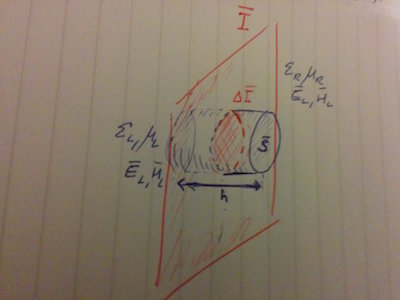
\includegraphics[height=0.3\textheight]{Figures/Chapters/PhysicalProblem/interfaceEPillBox}
  \end{center}
  \caption{Schematic showing integration surfaces used to obtain conditions for
    normal fields across an material interface.}
  \label{fig:material-interface-derivation:E-pillbox}
\end{figure}
In the limit $h \to 0$, all electric flux leaves the volume through the parallel
planes of the surface $S$, and~\eqref{eq:maxwell-gauss-integral} can be written
as
$$
\D_L \cdot \hat{\mathbf{n}} \Delta I - \mathbf{D}_R \cdot \hat{\mathbf{n}}
\Delta I = \rho_s \Delta I,
$$
where we have assumed that $S$ is sufficiently small that $D$ is constant. The
material interface condition can be written as
$$
\D_L \cdot \hat{\mathbf{n}} - \mathbf{D}_R \cdot \hat{\mathbf{n}} = \rho_s .
$$
Note that in the case where $\rho_s = 0$, meaning that there are no free
(unbound) charges, then the normal component of the electric flux density, $D$,
is continuous across the interface. By following the analogous procedure for the
magnetic field using~\eqref{eq:maxwell-gauss-magnetism-integral} we obtain
$$
\B_L \cdot \hat{\mathbf{n}} = \B_R \cdot \hat{\mathbf{n}} .
$$
These conditions are used with Maxwell's divergence equations.
% not used in the code!?

\subsection{Tangental fields}

Similarily for the tangental component of electric field we consider a closed
rectangular integration path in the plane of $\E_L$ and $\E_R$ around the same
interface, as shown
in~\eqref{fig:material-interface-derivation:E-rectangular-loop}. Again in the
limit $h \to 0$ and noting that $d\maxwellSource = 0$, we can
write~\eqref{eq:maxwell-faraday-integral} as
\begin{figure}[htbp!]
  \begin{center}
    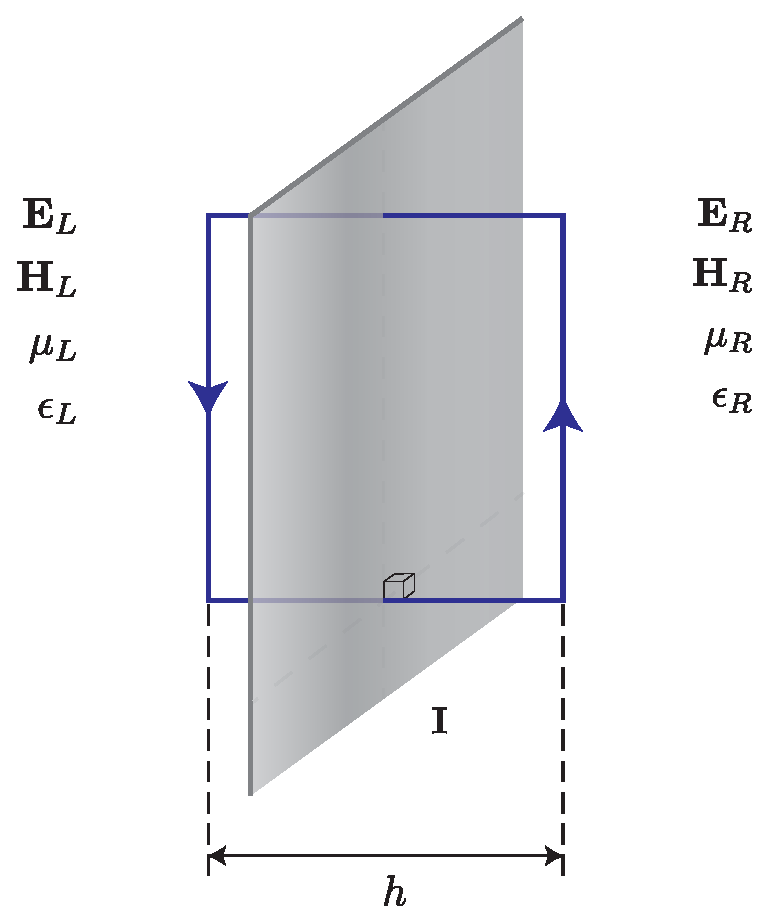
\includegraphics[height=0.3\textheight]{Figures/Chapters/PhysicalProblem/interfaceContour}
  \end{center}
  \caption{Schematic showing integration contours used to obtain conditions for
    tangental fields across an material interface.}
  \label{fig:material-interface-derivation:E-rectangular-loop}
\end{figure}
\begin{equation}
  \label{eq:material-interfaces-tangentalcondition-E}
  \int_{L_1}^{L_2} \E_L \cdot d\mathbf{l} - \int_{R_1}^{R_2} \E_R \cdot d \mathbf{l} = 0
\end{equation}
or
$$
\E_L \cdot d\mathbf{l} = \E_R \cdot d \mathbf{l} .
$$

The resulting interface condition is therefore that components of $\E$ tangental
to the interface are continuous - which can be written more generally as
$$
\hat{\mathbf{n}} \times \E_L = \hat{\mathbf{n}} \times \E_R .
$$
Again following an analogous procedure for the magnetic field we obtain
$$
\hat{\mathbf{n}} \cdot \H_L = \hat{\mathbf{n}} \times \H_R .
$$
These conditions are used with Maxwell's curl equations.

\subsection{Perfect electric conductors}
Metals with a large number of conduction band electrons can be described by the
perfect electric conductor (PEC) approximation. In a PEC the coulomb repulsion
between electrons causes all free charges to be distributed in an
infinitesimally thin layer on the surface of the material. The distribution of
free charges within a PEC changes instantaneously to counteract any applied
electric fields. Let us consider that the material on the right hand side of the
interface described above is a PEC. In this case, since $E_R$ is zero inside the
material, then~\eqref{eq:material-interfaces-tangentalcondition-E} simply
becomes
$$
\int_{L_1}^{L_2} \E_L \cdot d\mathbf{l} = 0 ,
$$
and the resulting condition is
$$
\E_L \times \hat{\mathbf{n}} = 0 .
$$
Similarily for the magnetic field we obtain
$$
\H_L \times \hat{\mathbf{n}} = \J_s ,
$$
% what about the other two conditions i.e. divergence conditions - should I
% specify those too?
where $\J_s$ is the surface current.

\subsection{Radiation condition}
Solution of many problems of interest require computation of phenomena occuring in a physical domain of infinite extent. In such a domain, electromagnetic sources should scatter energy to infinity. The inverse process, where radiation transfers energy from infinity to location of the sources is non-physical. To ensure uniqueness of solutions in an infinite domain, the following condition, known as the Silver-M\"uller radiation condition, should be satisfied
\begin{align}
\lim{ r \to \infty } \left( \xbf \times \left( \nabla \times \E \right) + \norm{\xbf} \dpartt{\E} \right) = 0, \\
\lim{ r \to \infty } \left( \xbf \times \left( \nabla \times \H \right) + \norm{\xbf} \dpartt{\H} \right) = 0.
\end{align}

\section{Relation to wave equation and Helmholtz equation}
\subsection{Wave equation}

Within a homogenous medium, where material parameters are constant and no free
currents or charges are present, Maxwell's equations can be written in wave
equation form, for which plane wave analytical solutions can be
obtained\cite{Jackson:490457}. By combining Faraday's law in SI
form,~\eqref{eq:maxwell-ampere}, with the appropriate constitutive equations for
non-dispersive media,~\eqref{eq:constitutive-linear}, we obtain the expression
\begin{equation}
  \label{eq:wave-equation-derivation-1}
  \nabla \times ( \nabla \times \H ) + \eps_0 \eps_r \dpartt{ \nabla \times \E } = 0 .
\end{equation}
where in the absence of free currents and charges we have used $\J = 0$ and
$\rho = 0$.

Subsituting both the vector identity $ \nabla \times ( \nabla \times \H ) = \nabla \cdot ( \nabla \cdot \H ) - \nabla^2 \H,
$
where we note from~\eqref{eq:maxwell-gauss-2} that $\nabla \cdot \H = 0$, and
Ampere's law,shown in~\eqref{eq:maxwell-ampere},
into~\eqref{eq:wave-equation-derivation-1} we obtain

\begin{equation}
  \label{eq:maxwell-wave-eqtn-H}
  \nabla^2 \H = \frac{1}{c^2} \ddpartt{ \H },
\end{equation}
which is a wave equation in the unknown $\H$, with the speed of the resultant wave given by $c_0 = 1/\sqrt{\eps_0 \eps_r \mu_0 \mu_r }$. We note that
the quantities $\eps_0$ and $\mu_0$ are related to the speed of light 
in vacuum $c_0 = 1/\sqrt{\eps_0 \mu_0 }$. A similar procedure can be followed, starting from
Ampere's law, leading to
\begin{equation}
  \label{eq:maxwell-wave-eqtn-E}
  \nabla^2 \E = \frac{1}{c^2} \ddpartt{ \E } .
\end{equation}
% TODO - Ruben : comments are missing - what are the advantages/limitations of
% this formulation!! Look at LeVeque - why do we use conservation laws in this
% way?

\subsection{Helmholtz equation}
The Helmholtz or reduced wave equation form of~\eqref{eq:maxwell-wave-eqtn-E} is
of particular interest for frequency domain numerical simulations. In this
approach the fields $\E$ and $\H$ are assumed to be time-harmonic, and are
expressed as
\begin{align}
  \label{eq:maxwell-helmholtz-time-harmonic}
  \E(\xbf,t) = \Re \left( \EHelm(\xbf) e^{i \omega t} \right), \\
  \H(\xbf,t) = \Re \left( \HHelm(\xbf) e^{i \omega t} \right),
\end{align}

which, by substitution into the wave equations given
in~\eqref{eq:maxwell-wave-eqtn-E} and~\eqref{eq:maxwell-wave-eqtn-H} we obtain
the Helmholtz equations for electric and magnetic fields
\begin{align}
  \label{eq:helmholtz}
  \nabla^2 \E(\xbf) + k^2 \E(\xbf) = 0, \\
  \nabla^2 \H(\xbf) + k^2 \H(\xbf) = 0,
\end{align}
where $k^2 =\omega^2/c^2$, is known as the propagation constant.

In this form the equations for $\E$ and $\H$ can be solved independently for
each angular frequency, $\omega$. This approached is best suited
to problems with a small number of frequencies of interest, for example a system
which is being driven at a known frequency. By contrast time domain approaches
allow solution for a broad band of frequency responses at once.


% TODO Balanis citation is incomplete P Drude - needs to be removed - maybe the
% solid state one (Optical properties of solids) instead Maybe swap some of the
% references for others (e.g. Fox) Ruben made LOADS of comments on citations Use
% some citations from Rubens paper also


%%% Local Variables:
%%% mode: latex
%%% TeX-master: "../Thesis"
%%% End:
